\documentclass[11pt]{article}

\usepackage[a4paper,margin=2.5cm]{geometry}
\usepackage[T1]{fontenc}
\usepackage[utf8]{inputenc}
\usepackage{lmodern}
\usepackage{cite}
\usepackage{amsmath,amssymb}
\usepackage{graphicx}
\usepackage{booktabs}
\usepackage{array}
\usepackage{microtype}
\usepackage[hidelinks]{hyperref}

\graphicspath{{images/}}

% Working manuscript for the next conference/journal submission.
% The content is intentionally written as a system-evaluation paper: it reports
% policy quality, runtime behavior, and dataset scale, without claiming causal
% learning gains before a classroom study.

\title{Policy-Guided Real-Time Mentoring for Introductory Programming: Design and Pilot Evaluation}
\author{Anonymized for double-blind review}
\date{}

\begin{document}

\maketitle

\begin{abstract}
First-year programming courses expose a practical weakness in many digital learning environments: students receive compiler messages and failed tests quickly, but they often do not receive help that is timely, limited, and safe for learning. A beginner who is debugging a loop boundary, a condition, or a missing statement ending may need a small nudge that keeps the solution in their hands, not a generated answer. This paper presents SocratesAI, a real-time virtual mentor for introductory programming that separates feedback action selection from feedback wording. The system analyses code states, keeps a compact session state, and applies a pedagogical policy before producing any student-facing message. The policy selects one of four actions: code-region highlight, conceptual hint, guiding question, or no feedback. A language model is used only after this action is selected, so it realizes a bounded intervention instead of deciding the tutoring strategy by itself. The prototype was evaluated through a real-HTTP PostgreSQL replay, a concurrent stress test, a rubric-labelled 12-problem suite, a 381,003-row weak-label policy dataset, model comparison with ablations, and a fixed end-to-end ML+Gemini benchmark. In the real-HTTP replay, 570 requests completed with mean latency of 44.11 ms and P95 latency of 58 ms; under eight-way concurrent load, all 400 requests completed with P95 latency of 56 ms. In the latest valid ML+Gemini run, the system processed 360 problem-suite events across 12 programming tasks with 0 runtime errors, 95.83\% agreement with target feedback actions, 95.80\% macro F1, mean latency of 1079.21 ms, and P95 latency of 2072 ms. A model comparison over the expanded dataset showed that removing analyzer-derived features reduced macro F1 from 1.0000 to 0.8813, which supports the role of structured code-analysis signals in the policy layer. These results should be read as system-level and policy-quality evidence, not as proof of learning gains. They show that bounded, policy-guided feedback can be implemented as a fast and auditable alternative to unconstrained LLM assistance.
\end{abstract}

\noindent\textbf{Keywords:} introductory programming, CS1, programming education, real-time feedback, virtual mentor, student modeling, pedagogical policy, AI-assisted learning

\section{Introduction}

Introductory programming is usually described as a difficult course because students must learn syntax, algorithms, and problem solving at the same time. That description is correct, but it misses one everyday detail of CS1 practice. Many students are not blocked by a large conceptual gap at first. They are blocked by a small mistake that appears at the wrong moment: a condition written in the wrong direction, a loop boundary that skips one value, a variable that is updated in the wrong place, or a test failure that seems unrelated to the code they just changed. If feedback comes only after submission, the student may already have built a wrong explanation of the problem.

Large classes make this situation harder. A teaching assistant can often diagnose the issue in a short conversation, but such conversations do not scale to every edit made during a lab session. Automated assessment systems fill part of the gap by checking syntax, running tests, and reporting correctness. The difficulty is that this feedback is usually thin. It can say that the answer is wrong, but it rarely decides whether the student needs a nudge, a conceptual reminder, a question, or no interruption at all \cite{NavigatingAutomatedFeedback,AutomatedGradingandFeedbackToolsforProgrammingEducationSystematicReview}.

Recent AI-based tools have changed expectations. Students now know that a conversational system can explain a program, suggest a fix, and produce code in a few seconds. Systems such as CodeAid, Iris, and CS50's AI assistant show that this kind of support can be integrated into programming education at scale \cite{CodeAid,IRIS,ImprovingAIinCS50}. The same line of work also shows the risk. If help is too direct, students may ask for the next step instead of reasoning through the error. If help is fluent but wrong, it can be more persuasive than a compiler message. If the tool is always available and always verbose, it may train students to depend on it \cite{PatternsofLLMPoweredProgrammingAssistant,FeasibilityStudyofAugmentingTeachingAssistantswithAI,SystematicLiteratureReviewonLLM}.

This paper takes a simple position: the central problem is not only how to generate feedback, but how to decide what kind of feedback should be given at a particular moment. For that reason, the virtual mentor described here is not designed as an open chat assistant. It is implemented as a decision pipeline. The analyzer reads the current code state, the profile manager tracks a small amount of session history, the policy layer chooses a feedback action, and the realization layer turns that action into a short response or interface cue. The language model, when used, is deliberately placed after the policy decision.

The study addresses two research questions:

\begin{itemize}
\item \textbf{RQ1:} Can a policy-guided mentor operate within an interactive latency range during introductory programming practice?
\item \textbf{RQ2:} How well does the policy layer select rubric-aligned feedback actions on programming problem states when it is executed as a real service?
\item \textbf{RQ3:} Which groups of features are most important for learning the feedback-action policy from exported mentoring data?
\end{itemize}

The contribution of the paper is fourfold. First, it gives a concrete architecture for in-process programming feedback, with a clear separation between code analysis, learner state, policy selection, and message realization. Second, it explains how a small policy model can regulate feedback detail instead of relying on unconstrained natural-language generation. Third, it reports a larger and clearer evaluation artifact than the previous version of this work: a 1,080-row rubric problem-suite dataset, a 381,003-row weak-label policy dataset, a live 360-event ML+Gemini benchmark, and model comparisons across rule, logistic regression, random forest, XGBoost, LightGBM, and a small neural classifier. Fourth, it states the boundary of the evidence explicitly: the current results support technical feasibility and action-selection validity, while learning-gain claims still require a classroom study.

\section{Literature Review}

\subsection{Feedback in introductory programming}

Feedback in programming education has to do more than mark an answer as correct or incorrect. A beginner needs to connect a visible symptom, such as a compiler error or a failed test, with an underlying cause in the program. This is difficult because the same symptom may come from different causes. A failed test in a two-sum task, for example, may point to an indexing mistake, a misunderstanding of hash-map lookup, or a wrong assumption about duplicate values. A generic message does not help the student distinguish between these cases.

Automated assessment systems are valuable because they reduce waiting time and grading load. Reviews of automated grading and feedback tools show that unit tests, static analysis, compiler diagnostics, and repair systems can support large-scale programming courses \cite{AutomatedGradingandFeedbackToolsforProgrammingEducationSystematicReview,NavigatingAutomatedFeedback}. However, the same reviews also report a recurring limitation: feedback is often tied to correctness rather than to the student's current reasoning process. For CS1 students, this distinction matters. They need feedback that is short enough to keep the coding flow intact and specific enough to prevent random trial-and-error.

\subsection{Intelligent tutoring and student modeling}

Intelligent tutoring systems address this problem by modeling the learner and adapting support. In programming education, tutor systems can track repeated errors, misconceptions, progress through subgoals, and task attempts. Adaptive systems such as AIF 3.0 show that immediate feedback can be designed around subgoals rather than only final correctness \cite{AdaptiveImmediateFeedbackforBlockBasedProgramming}. Broader work on AI tutoring also emphasizes that adaptivity must be understandable to teachers, because instructors need to know what kind of help students receive \cite{AITutoringinSDEducation,AIEnabledIntelligentAssistant}.

The virtual mentor in this study uses a deliberately small student model. It does not try to infer a complete knowledge state. Instead, it records signals that are useful during a short programming session: repeated error type, number of previous interventions, last feedback action, whether the last action helped, suspicious code region, and attempt number. This choice keeps the model transparent. It also reduces the amount of data needed before the system can make a decision.

\subsection{LLM-based programming assistants}

Large language models are attractive for programming education because they can explain code in ordinary language and respond flexibly to student questions. Studies of LLM-based feedback and tutoring show promising results, especially when the system is constrained by instructional rules \cite{CodeAid,IRIS,AutomatingHumanTutorStyleProgrammingFeedback,EvaluationofLLMtoolsforfeedbackgeneration}. CodeAid is particularly relevant because it tries to balance student help with educator control, while Iris shows how a virtual tutor can be embedded into computer science learning contexts.

The open issue is control. A language model can produce a useful explanation, but it can also reveal too much, introduce an error, or answer a question that the course intentionally wants students to solve themselves. Studies of help-seeking behavior with LLM-powered assistants show that students do not always use such tools in ways that support learning \cite{PatternsofLLMPoweredProgrammingAssistant}. This does not mean that language models should be excluded from CS1. It means that the model should not be the only component deciding the mentoring strategy.

\subsection{Research gap}

The systems discussed above address important parts of the problem, but three requirements are not always combined in one design. The first is in-process feedback: help should be available while the code is being written, not only after a final submission. The second is a lightweight student state: repeated difficulty should change the feedback action, even if the current code error looks similar. The third is policy-level control: the system should be able to choose silence, a highlight, a hint, or a question before generating text.

The proposed mentor is built around these three requirements. It is not meant to replace an instructor or to compete with full tutoring systems. It is a middle layer between automated checks and human teaching: fast enough to support live practice, constrained enough to avoid solution disclosure, and explicit enough for later classroom evaluation.

\section{System Design}

\subsection{Design principles}

The prototype was built around four design principles. First, feedback should be \emph{timely}. If the system waits several seconds, the student may already have changed the code and the intervention becomes detached from the original mistake. Second, feedback should be \emph{limited}. A novice does not always need a paragraph; sometimes a highlighted line is enough. Third, feedback should be \emph{traceable}. The reason for an intervention should be visible in analyzer and policy signals, not hidden entirely inside a generated response. Fourth, feedback should be \emph{safe for learning}. The system should avoid writing the final solution for the student.

These principles led to the architecture shown in Fig.~\ref{fig:architecture}. The front end sends code states to the backend, where the mentor workflow orchestrator coordinates analysis, profile updates, policy selection, and feedback realization. The policy inference service is separated from the main backend so that rule-based and learned policies can be compared without changing the user interface.

\begin{figure}[htbp]
\centering
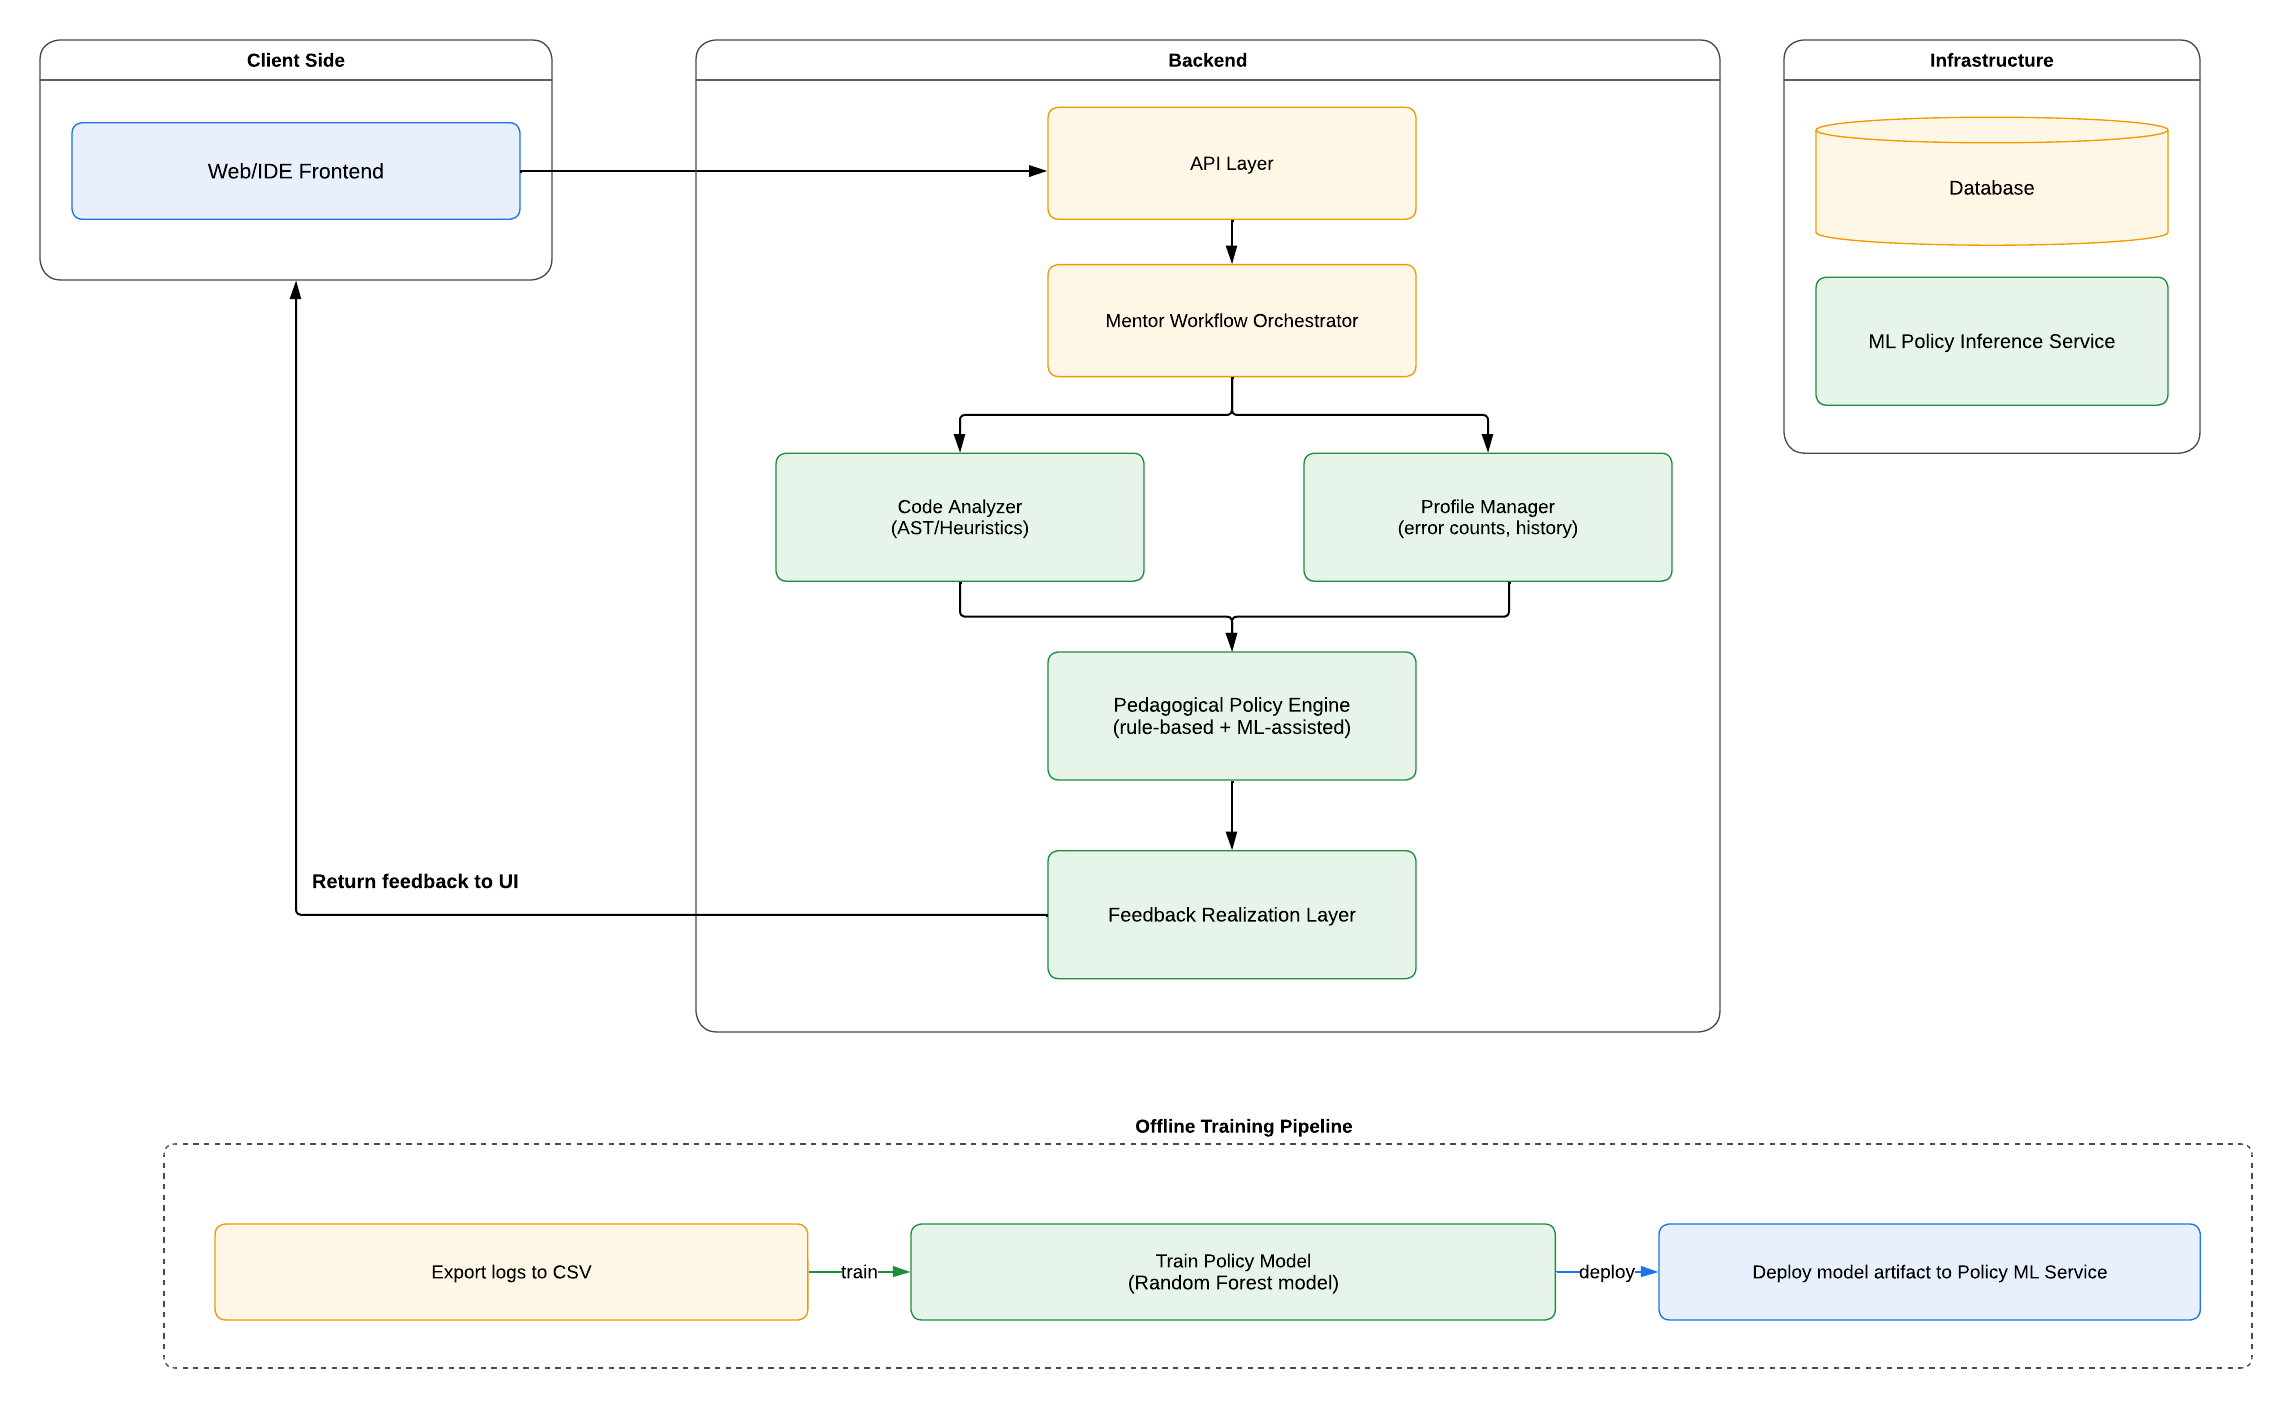
\includegraphics[width=\linewidth]{arch-SIST.png}
\caption{System architecture of the virtual mentor, including the real-time mentoring loop and the offline policy-training pipeline.}
\label{fig:architecture}
\end{figure}

\subsection{Analyzer and learner state}

The analyzer converts a code snapshot into a compact set of signals. In the current prototype these signals include compile status, number of passed and failed tests, error type, severity, code length, suspicious region, and approximate task progress. The analyzer is intentionally heuristic. It is not expected to understand every possible student program. Its purpose is to provide enough structure for a mentoring decision.

The learner state is also compact. It records the number of times the same error has appeared, the total number of recent errors in the session, the previous feedback action, whether the previous action was marked as helpful, and how many interventions have already been given. This state is not a full cognitive model. It is closer to what a teaching assistant may keep in mind during a short lab conversation: ``this student has already seen this error twice'' or ``a direct hint was given recently, so the next intervention should be lighter.''

\subsection{Policy layer}

The policy layer selects one of four feedback actions:

\begin{itemize}
\item \texttt{CODE\_HIGHLIGHT}: the interface points to a suspicious region while giving little explanation.
\item \texttt{CONCEPTUAL\_HINT}: the system gives a brief reminder about the relevant programming idea.
\item \texttt{GUIDING\_QUESTION}: the system asks a question intended to make the student inspect their own code.
\item \texttt{NO\_FEEDBACK}: the system stays silent because intervention is not useful or the evidence is weak.
\end{itemize}

The distinction between these actions is pedagogically important. A code highlight is useful when the location of the problem is more important than the explanation. A conceptual hint is useful when the student appears to be missing a concept. A guiding question is useful when the system should slow the student down and prompt reasoning. No feedback is useful when an interruption would only add noise.

Formally, the analyzer maps a code state $c_t$ into an event descriptor $e_t$. The profile manager maintains a session state $s_t$, and the policy chooses an action $a_t$:

\[
\pi(e_t, s_t) \rightarrow a_t,\quad a_t \in \{\texttt{CODE\_HIGHLIGHT}, \texttt{CONCEPTUAL\_HINT}, \texttt{GUIDING\_QUESTION}, \texttt{NO\_FEEDBACK}\}.
\]

This formulation is simple, but it is useful because it separates the policy decision from the wording of the message. The same action can later be realized by templates, by a language model, or by a teacher-authored feedback bank.

\subsection{Learned policy extension}

The prototype includes both a rule-based policy and a learned policy extension. The learned policy is a multi-class Random Forest classifier implemented with \texttt{scikit-learn}. The model uses features available at runtime: error type, severity, compile result, test results, recurrence counts, attempt number, last feedback action, last feedback success, suspicious-region flag, code length, and total feedback count in the session. It predicts the same four action labels used by the rule-based policy.

The classifier used 200 trees and a maximum depth of 8. Leaf nodes required at least two samples, class weights were balanced by subsample, and the random seed was fixed at 42. The preprocessing pipeline imputes missing categorical values, one-hot encodes categorical features, imputes booleans with the most frequent value, and imputes numeric fields with the median.

Two model-development datasets were used. The larger dataset contains 381,003 weakly labelled policy examples derived from 117,232 coding sessions in the local programming-problem corpus. It is used as a scale check: the question is whether the exported runtime features can reproduce a deployable feedback-action policy across many problem states. A second 1,080-row dataset was built from the real-HTTP problem-suite log; in that dataset, the target label is the review-rubric action for the code state. Together, these datasets exercise the full policy pipeline: syntax failures, loop-boundary mistakes, condition mistakes, unfinished attempts, repeated conceptual errors, and locally complete states.

The model-development study compared a rule baseline, logistic regression, random forest, XGBoost, LightGBM, and a small neural classifier. It also included feature ablations that removed history features, analyzer features, suspicious-region information, and the last feedback action. This comparison is important for the technical depth of the work. It shows that the mentor is not only an LLM wrapper: the structured analyzer and session features are measurable parts of the policy. In this version, the learned policy is treated as a deployable extension of the rule policy rather than as the main pedagogical claim. The more important question is whether it preserves intended intervention behavior on problem-level code states and whether it can be evaluated cleanly against rubric labels.

\subsection{Interface}

Fig.~\ref{fig:interface} shows the main interface elements used during a programming session. The student sees the task card, code editor, mentor feedback panel, analyzer metadata, and feedback-loop controls. The feedback-loop controls are included because the prototype needs explicit outcome labels. When a learner marks feedback as helpful or still insufficient, the interaction log can store whether the intervention was resolved after feedback and how long the fix took.

\begin{figure}[htbp]
\centering

\includegraphics[width=\linewidth,trim=0 0 0 70,clip]{interface.png}
\caption{Annotated mentor interface used in the pilot sessions. The identifying header area is omitted in the review draft.}
\label{fig:interface}
\end{figure}

\section{Methodology}

\subsection{Research design}

The study follows a prototype-based evaluation design. The immediate goal was to examine whether the mentoring loop can operate during live coding, whether the policy layer selects rubric-aligned actions, and whether the exported logs are rich enough for later classroom research. A controlled learning-gain study is outside the scope of this paper.

The first runtime artifact contains 570 event-level records generated by a deterministic replay of introductory programming scenarios through a real Spring Boot HTTP process. The service used the same authenticated mentor endpoint as the application and stored state in a PostgreSQL 16.11 database running through Docker Compose. Feedback realization used templates, and the replay used the rule-based policy selector. This artifact was used mainly to test low-latency operation of the backend mentoring loop.

The second runtime artifact is the current primary problem-suite benchmark. It used 12 programming tasks: palindrome checking, two-sum, valid parentheses, binary search, merge sorted array, trapping rain water, LRU cache, longest substring without repeating characters, reverse linked list, matrix diagonal sum, Roman-to-integer conversion, and climbing stairs. Each problem was replayed across five fresh cohorts as a six-step coding sequence: syntax issue, unfinished implementation, first conceptual mistake, repeated conceptual mistake, partial compiling logic, and local completion. The benchmark used the ML policy service through FastAPI, PostgreSQL-backed session state, and Gemini 2.5 Flash-Lite for feedback realization. Fresh synthetic student identifiers were used so that history features from earlier runs could not contaminate the state.

The third artifact is the model-development data. The rubric problem-suite dataset contains 1,080 rows and uses \texttt{target\_feedback\_action} as the supervised label. The expanded weak-label dataset contains 381,003 rows derived from 117,232 coding sessions and uses \texttt{feedback\_action} as the target. The weak-label dataset is not treated as expert classroom evidence. It is used to test scale, compare classifiers, and run feature ablations.

The unit of analysis is therefore the event, not the student. This distinction is important. Event-level analysis can show whether the system responds quickly and whether the policy produces a plausible distribution of feedback actions under repeated scenario patterns. The problem-suite benchmark can show whether the running ML+LLM pipeline matches rubric action labels. It cannot by itself show that students learned more, retained concepts longer, or transferred debugging skill to new tasks.

\begin{table}[htbp]
\centering
\caption{Evaluation artifacts used in the study}
\label{tab:evaluation_artifacts}
\small
\renewcommand{\arraystretch}{1.15}
\begin{tabular}{p{0.34\textwidth} p{0.14\textwidth} p{0.42\textwidth}}
\toprule
\textbf{Artifact} & \textbf{Size} & \textbf{Purpose} \\
\midrule
Real-HTTP replay & 570 events & Backend responsiveness and stable template-based mentoring loop \\
Concurrent smoke test & 400 requests & Stability under eight-way parallel load \\
Fixed ML+Gemini problem suite & 360 events & End-to-end action quality and LLM feedback realization \\
Rubric policy dataset & 1,080 rows & Supervised target-action evaluation on problem states \\
Expanded weak-label dataset & 381,003 rows & Classifier comparison and feature ablation at larger scale \\
\bottomrule
\end{tabular}
\end{table}

\subsection{Logged variables}

Each event can be written as

\[
x_i = (e_i, r_i, h_i, a_i, t_i, o_i),
\]

where $e_i$ is the error descriptor, $r_i$ is the recurrence information, $h_i$ is recent feedback history, $a_i$ is the selected action, $t_i$ is the latency vector, and $o_i$ is the observed outcome. The latency vector contains analysis time, policy time, feedback-realization time, and platform overhead:

\[
T_{total}=T_{analysis}+T_{policy}+T_{feedback}+T_{overhead}.
\]

Table~\ref{tab:variables} summarizes the main variables used in the pilot analysis.

\begin{table}[htbp]
\centering
\caption{Main variables captured in the event-level log}
\label{tab:variables}
\small
\renewcommand{\arraystretch}{1.15}
\begin{tabular}{p{0.27\textwidth} p{0.63\textwidth}}
\toprule
\textbf{Variable group} & \textbf{Examples} \\
\midrule
Analyzer state & Error type, severity, compile success, tests passed, tests failed, suspicious code region, code length \\
Session state & Same-error count, total errors seen, attempt number, last feedback action, last feedback success \\
Policy output & Selected action, policy version, feedback source, feedback version \\
Timing & Analysis time, policy time, feedback realization time, total latency \\
Operational status & Request success, direct-solution violation flag \\
\bottomrule
\end{tabular}
\end{table}

\subsection{Metrics}

Three groups of metrics were used. The first group measures responsiveness: mean request latency, P95 latency, P99 latency, replay throughput, and stress-test completion under concurrent load. These metrics matter because the mentor is intended for active coding, where feedback that arrives too late can disrupt the student's flow.

The second group measures action-selection behavior: the number and share of code highlights, conceptual hints, guiding questions, and no-feedback decisions in the replay. The third group measures policy quality on the 12-problem suite using action agreement, macro F1, per-class precision, recall, F1, per-problem agreement, and runtime errors. Action agreement is the share of events where the selected feedback action matches the review-rubric action label. The benchmark also records feedback source, which makes it possible to distinguish Gemini responses from deterministic template fallbacks. The fourth group checks the model-development pipeline with classifier accuracy, macro F1, per-class metrics, and ablation results. These metrics are useful for checking whether the mentoring pipeline behaves consistently, but they are not substitutes for student learning-outcome measures.

\section{Results}

\subsection{Backend responsiveness}

The prototype remained within the intended interactive range in the real-HTTP PostgreSQL replay. Across the 570 replayed events, all requests completed successfully. The mean request-level latency was 44.11 ms, the median was 46 ms, the P95 latency was 58 ms, and the P99 latency was 68 ms. The replay completed in 25.151 s, corresponding to 22.66 requests per second on the local evaluation machine. The analyzer time reported by the service averaged 6.81 ms, with P95 of 10 ms.

\begin{table}[htbp]
\centering
\caption{Real replay responsiveness test results from the event-level records}
\label{tab:latency_results}
\renewcommand{\arraystretch}{1.15}
\begin{tabular}{lcc}
\toprule
\textbf{Metric} & \textbf{Request latency} & \textbf{Analyzer time} \\
\midrule
Mean & 44.11 ms & 6.81 ms \\
Median & 46 ms & 7 ms \\
P95 & 58 ms & 10 ms \\
P99 & 68 ms & 17 ms \\
\bottomrule
\end{tabular}
\end{table}

For a programming mentor, these values are more than technical performance numbers. They shape the kind of pedagogy the system can support. A slow assistant tends to become a separate help channel, similar to asking a forum or chatbot. A faster mentor can behave more like a lab assistant who quietly points to the current problem while the student is still thinking about it.

The same real-HTTP harness ran an additional concurrent smoke test with 400 authenticated mentor requests at concurrency level 8. All requests completed successfully. The P95 latency was 56 ms and the P99 latency was 61 ms. This result does not represent production capacity planning, because it is a local single-machine benchmark, but it gives evidence that the request pipeline remains stable under modest parallel load when backed by PostgreSQL.

\begin{table}[htbp]
\centering
\caption{Concurrent stress smoke test}
\label{tab:stress_results}
\renewcommand{\arraystretch}{1.15}
\begin{tabular}{lc}
\toprule
\textbf{Metric} & \textbf{Value} \\
\midrule
Requests & 400 \\
Concurrency & 8 \\
Errors & 0 \\
Wall time & 1.894 s \\
Throughput & 211.19 requests/s \\
Mean latency & 37.59 ms \\
P95 latency & 56 ms \\
P99 latency & 61 ms \\
\bottomrule
\end{tabular}
\end{table}

\subsection{Action-selection behavior in the template replay}

Table~\ref{tab:action_distribution} shows the action distribution produced by the 570-event template replay. Conceptual hints were the most frequent action, followed by code highlights, guiding questions, and no-feedback decisions. This distribution is consistent with the policy design: repeated errors tend to escalate from highlighting to conceptual support, unfinished implementation states are handled as guiding-question opportunities, and locally complete snippets produce no feedback.

\begin{table}[htbp]
\centering
\caption{Policy action distribution in the event replay}
\label{tab:action_distribution}
\renewcommand{\arraystretch}{1.15}
\begin{tabular}{lcc}
\toprule
\textbf{Action} & \textbf{Events (N)} & \textbf{Share} \\
\midrule
\texttt{CODE\_HIGHLIGHT} & 90 & 15.79\% \\
\texttt{CONCEPTUAL\_HINT} & 330 & 57.89\% \\
\texttt{GUIDING\_QUESTION} & 90 & 15.79\% \\
\texttt{NO\_FEEDBACK} & 60 & 10.53\% \\
\bottomrule
\end{tabular}
\end{table}

The replay also showed why the four-action policy is useful. Code highlights and conceptual hints are suitable when the student is close to a repair and needs orientation. Guiding questions are slower by design; they ask the student to inspect the program rather than immediately apply a suggested change. The \texttt{NO\_FEEDBACK} action is also necessary. Without it, the system would treat every analyzer signal as a reason to interrupt, which is not how a human tutor behaves.

\subsection{Fixed ML+Gemini problem-suite benchmark}

The strongest current runtime evidence comes from the fixed ML+Gemini problem-suite benchmark. The system processed 360 events across 12 programming problems and five fresh cohorts. All 360 requests completed successfully, and there were no policy-service or LLM-provider runtime errors in the benchmark output. The policy action matched the target rubric action in 95.83\% of events, with macro F1 of 95.80\%. Mean end-to-end wall latency was 1079.21 ms and P95 latency was 2072 ms. In this run, 317 responses were produced by Gemini and 43 used the deterministic template fallback.

\begin{table}[htbp]
\centering
\caption{Fixed ML+Gemini benchmark on the 12-problem suite}
\label{tab:fixed_ml_gemini}
\small
\renewcommand{\arraystretch}{1.15}
\begin{tabular}{lc}
\toprule
\textbf{Metric} & \textbf{Value} \\
\midrule
Events & 360 \\
Successful requests & 360 \\
Runtime errors & 0 \\
Action agreement & 95.83\% \\
Macro F1 & 95.80\% \\
Mean latency & 1079.21 ms \\
P95 latency & 2072 ms \\
Gemini responses & 317 \\
Template fallbacks & 43 \\
\bottomrule
\end{tabular}
\end{table}

\begin{figure}[htbp]
\centering
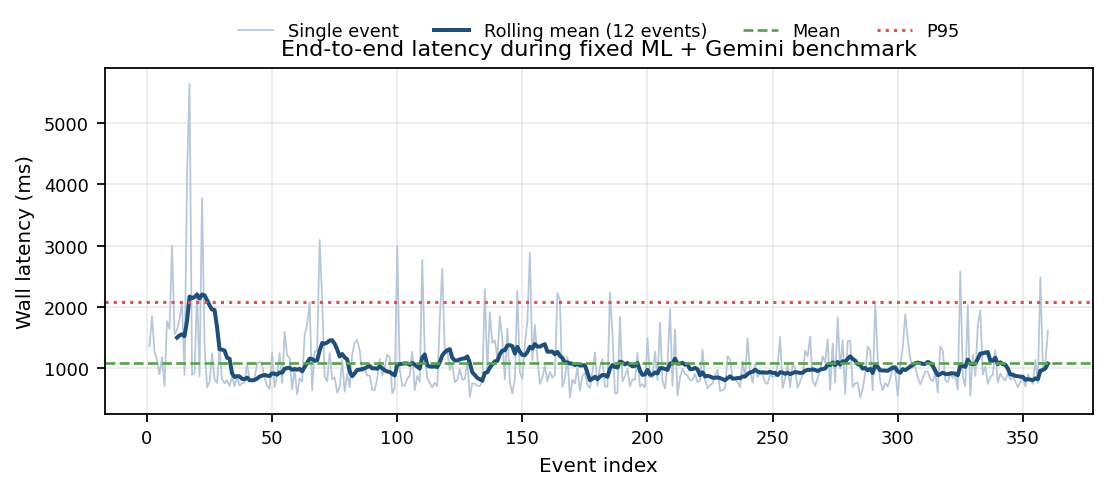
\includegraphics[width=0.95\linewidth]{sist_latency_timeline.png}
\caption{End-to-end latency across the fixed ML+Gemini problem-suite benchmark. The rolling mean shows that most requests remained within a few seconds even when LLM realization was enabled.}
\label{fig:latency_timeline}
\end{figure}

The class-level results in Table~\ref{tab:per_class_fixed} show that the policy was strongest for guiding questions and code highlights. The lowest F1 was still \texttt{NO\_FEEDBACK}, at 90.91\%, because the system sometimes intervened in local-completion states where the expected action was silence.

\begin{table}[htbp]
\centering
\caption{Per-class action metrics in the fixed ML+Gemini benchmark}
\label{tab:per_class_fixed}
\small
\renewcommand{\arraystretch}{1.15}
\begin{tabular}{lcccc}
\toprule
\textbf{Action} & \textbf{Precision} & \textbf{Recall} & \textbf{F1} & \textbf{Support} \\
\midrule
\texttt{CODE\_HIGHLIGHT} & 95.24\% & 100.00\% & 97.56\% & 100 \\
\texttt{CONCEPTUAL\_HINT} & 93.10\% & 96.43\% & 94.74\% & 140 \\
\texttt{GUIDING\_QUESTION} & 100.00\% & 100.00\% & 100.00\% & 60 \\
\texttt{NO\_FEEDBACK} & 100.00\% & 83.33\% & 90.91\% & 60 \\
\bottomrule
\end{tabular}
\end{table}

\begin{figure}[htbp]
\centering
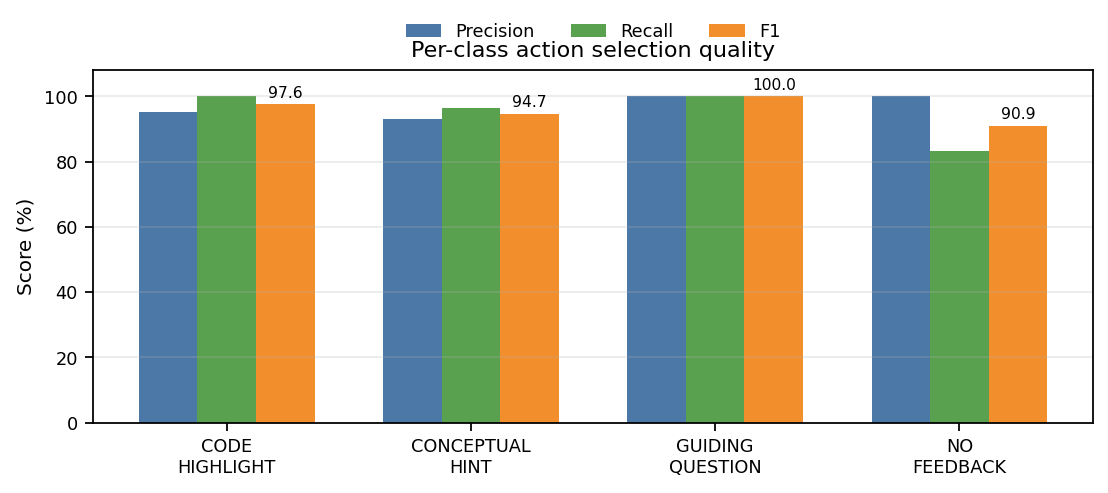
\includegraphics[width=0.92\linewidth]{sist_per_class_metrics.png}
\caption{Per-class precision, recall, and F1 in the fixed ML+Gemini benchmark.}
\label{fig:per_class_metrics}
\end{figure}

Problem-level agreement is shown in Fig.~\ref{fig:problem_agreement}. Ten of the twelve tasks reached 100\% action agreement. The two weaker tasks were \texttt{lru-cache} and \texttt{valid-parentheses}. In total, the benchmark had 15 disagreements: five in \texttt{lru-cache} first conceptual error states, five in \texttt{lru-cache} local completion states, and five in \texttt{valid-parentheses} local completion states. This pattern is useful because it gives a concrete next engineering target instead of only a general score.

\begin{figure}[htbp]
\centering
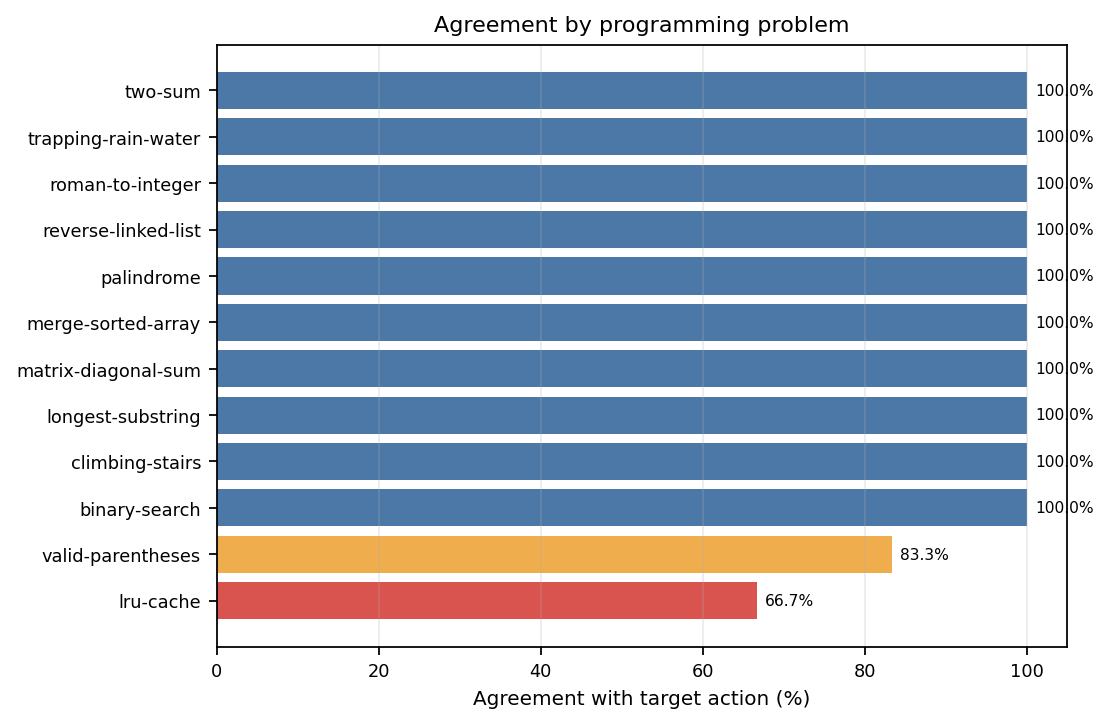
\includegraphics[width=0.95\linewidth]{sist_problem_agreement.png}
\caption{Agreement with target feedback action by programming problem.}
\label{fig:problem_agreement}
\end{figure}

\subsection{Model-development check}

The learned policy extension was trained on 381,003 model-development examples from the expanded weak-label policy dataset. The target was \texttt{feedback\_action}, so this experiment tested whether classifiers could reproduce the current deployable policy from exported runtime features. A problem-level group holdout produced 303,515 training rows and 77,488 test rows for the final Random Forest training run. The model reached 1.0000 accuracy and 1.0000 macro F1. This high score is expected because the labels are weak proxy labels derived from the current policy logic. It is useful as a scale and pipeline check, not as educational validation.

The second model check used the 1,080-row problem-suite policy dataset, where the label was the review-rubric action for each code state. A problem-level group holdout trained on 810 rows and tested on 270 rows from three held-out problems: binary search, trapping rain water, and two sum. The classifier reached 1.0000 action accuracy and 1.0000 macro F1 on this held-out split. This result shows that the review-rubric action labels are learnable from the same runtime features used by the mentor, but it is still reported as pipeline validation rather than as a learning-gain result.

The model-comparison study also gives a clearer technical answer to the question of what information matters. On the 381,003-row weak-label dataset, the compared classifiers all reproduced the policy with all features. When analyzer features were removed, the best observed scores dropped to 92.32\% accuracy and 88.13\% macro F1. Fig.~\ref{fig:ablation} summarizes this drop. The result supports the architectural decision to keep structured analyzer signals before LLM feedback realization.

\begin{figure}[htbp]
\centering
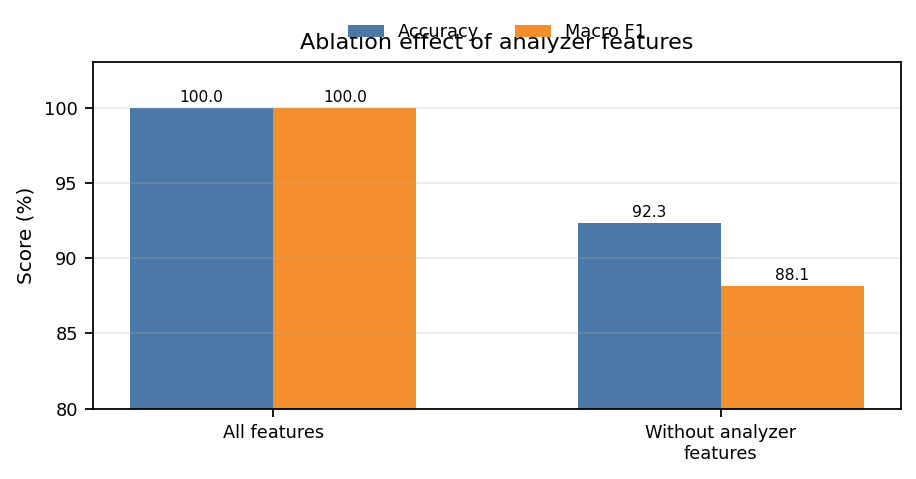
\includegraphics[width=0.8\linewidth]{sist_ablation_analyzer_features.png}
\caption{Ablation result on the expanded weak-label dataset. Removing analyzer features reduces macro F1, showing that structured code-analysis signals contribute to policy prediction.}
\label{fig:ablation}
\end{figure}

\subsection{Baseline context}

For context, an earlier deterministic 12-problem policy comparison showed that a fixed no-policy selector that always returns a conceptual hint reached only 38.89\% action agreement and 14.00\% macro F1. This baseline is intentionally simple, but it is important. It shows why the policy layer should not be removed: a generic hint can be correct for some repeated conceptual errors, but it cannot highlight code, ask a guiding question, or stay silent when intervention is unnecessary. The current fixed ML+Gemini benchmark improves the action-quality evidence while also testing the full feedback-realization path.

\section{Discussion}

\subsection{Why policy control matters}

The main lesson from the prototype is that real-time programming feedback should not be treated as a text-generation problem only. A generated explanation can be useful, but the prior decision is more important: should the system intervene at all, and if so, how explicit should the intervention be? This is the part of tutoring that many students experience as judgment. A teaching assistant does not always answer the same error in the same way; the assistant considers whether the student has seen the error before, whether the student is making progress, and whether a direct hint would remove the learning opportunity.

The policy layer gives the software a modest version of that judgment. It does not make the system intelligent in the human sense, but it prevents the feedback generator from being the only authority. This is especially important when language models are used. The policy can restrict the model to a guiding question or a short conceptual hint, instead of allowing it to produce a full solution.

\subsection{Engineering-pedagogy implications}

From an engineering-pedagogy perspective, the mentor is useful because it connects implementation detail with instructional control. The architecture does not hide pedagogy inside a black-box prompt. Teachers can inspect the available actions, change thresholds, disable direct hints during assessment, or require more guiding questions during practice. This makes the tool easier to align with a course policy.

The event log is also useful for instructors. A class-level summary can show which error types repeat, which tasks generate many hints, and where students keep asking for support. Such information can guide a teacher's next lab explanation or revision of task wording. In this sense, the mentor is not only a feedback tool for students; it can also become a diagnostic tool for course design.

\subsection{Limits of the current evidence}

The results should be interpreted as system-level and policy-level evidence. The latency, action-distribution, fixed ML+Gemini benchmark, and ablation study show that the mentoring loop is technically feasible and that the policy produces traceable actions across a broader set of programming tasks. They do not yet answer the learning question. Learning gains, retention, and transfer need a different design with student-level pre-tests, post-tests, delayed tasks, and comparison conditions.

\section{Study Limitations}

The main limitation is that this is still an instrumented prototype evaluation, not a semester-long classroom study. The new problem-suite benchmark is broader than the initial replay, because it includes tasks such as binary search, valid parentheses, trapping rain water, and LRU cache. However, the metrics are still interaction-level metrics. They show whether the system selects the intended type of feedback, not whether students improve their long-term programming skill.

There are also three technical limits. First, the analyzer remains intentionally lightweight. The remaining disagreements in \texttt{lru-cache} and \texttt{valid-parentheses} show that the system still needs better handling of local-completion and unknown-logic states. Second, the expanded 381,003-row dataset is weakly labelled, not expert-labelled classroom data. This is acceptable for scale testing and ablation, but it cannot replace reviewed instructor labels. Third, the benchmark records whether feedback came from Gemini or a template, but it does not yet separate fallback reasons such as timeout, provider error, empty response, or safety block.

\section{Future Research Directions}

Future work should move in three directions. The first is classroom evaluation. A larger study should compare policy-guided mentoring with ordinary automated feedback, fixed generic feedback, and unstructured chatbot help. The study should measure not only immediate fixes but also debugging confidence, conceptual understanding, delayed performance, and student reliance on the tool.

The second direction is policy validation. The learned policy should be retrained on reviewed interaction traces. A practical next step is to collect 200--500 manually reviewed events and ask two instructors or teaching assistants to label an overlapping subset of 50--100 events. This would make it possible to report inter-rater agreement, for example Cohen's kappa, and compare rule-based and learned policies against human pedagogical judgments rather than only proxy labels.

The third direction is teacher control. Instructors should be able to tune the feedback policy for different phases of a course. During early practice, conceptual hints may be appropriate. During graded labs, guiding questions and code highlights may be safer. During exam-like conditions, the mentor may need to record errors without intervening.

\section{Conclusion}

This paper presented SocratesAI, a policy-guided virtual mentor for introductory programming. The system separates analyzer signals, session-level student state, feedback action selection, and final feedback realization. This separation is the main design contribution: it keeps the mentoring behavior visible and allows the system to regulate help before any message is generated.

The evaluation gives stronger evidence than the earlier prototype version. The real-HTTP replay used 570 event-level records through a Spring Boot service backed by PostgreSQL and achieved mean request latency of 44.11 ms with P95 latency of 58 ms. In a concurrent stress test with 400 requests at concurrency 8, all requests completed successfully and P95 latency was 56 ms. The latest fixed ML+Gemini problem-suite benchmark processed 360 events across 12 tasks and five fresh cohorts with 0 runtime errors, 95.83\% agreement with target feedback actions, 95.80\% macro F1, mean latency of 1079.21 ms, and P95 latency of 2072 ms. The expanded weak-label dataset now contains 381,003 rows, and the ablation study shows that analyzer-derived features are important for policy prediction. These findings do not prove improved learning outcomes, but they do show that real-time, policy-guided feedback is technically feasible and that explicit action selection gives stronger behavior than generic feedback. The next step is a classroom study that connects event-level behavior with student-level learning.

\nocite{Francisco2022}
\nocite{Chrysafiadi2022}
\nocite{pankiewicz2023largelanguagemodelsgpt}
\nocite{AutomatedAssessmentToolsForGrading2022}
\nocite{AdaptiveImmediateFeedbackforBlockBasedProgramming}
\nocite{FeedbackSystemSupportingStudents2022}
\nocite{EvaluationofLLMtoolsforfeedbackgeneration}
\nocite{AutomatingHumanTutorStyleProgrammingFeedback}
\nocite{AITutoringinSDEducation}
\nocite{AutomatedGradingandFeedbackToolsforProgrammingEducationSystematicReview}
{\footnotesize
\bibliographystyle{IEEEtran}
\bibliography{references}
}

\end{document}
